\documentclass{article}

% DATA 275P report: NeurIPS 2025 style (preprint so authors are visible).
% Search for \pending to locate unfinished work.
% Figures may sit next to main.tex or inside a figures/ folder; both are found.
\usepackage[preprint]{neurips_2025}

\usepackage[utf8]{inputenc}
\usepackage[T1]{fontenc}
\usepackage{hyperref}
\usepackage{url}
\usepackage{booktabs}
\usepackage{amsfonts}
\usepackage{amsmath}
\usepackage{amssymb}
\usepackage{microtype}
\usepackage{xcolor}
\usepackage{graphicx}
\usepackage{array}
\usepackage{tabularx}
\usepackage{tikz}
\usetikzlibrary{arrows.meta,positioning}

\hypersetup{breaklinks=true,hidelinks}
\setlength{\emergencystretch}{1.5em}
\graphicspath{{./}{figures/}}

\newcommand{\pending}[1]{\textcolor{gray}{\textit{[To be completed: #1]}}}
\newcommand{\E}{\mathbb{E}}
\newcommand{\KL}{D_{\mathrm{KL}}}
\newcommand{\missing}{\textemdash}
\newcolumntype{Y}{>{\raggedright\arraybackslash}X}

% \figureorbox{file.png}{fallback text}: includes the image from ./ or figures/,
% otherwise draws a framed placeholder so the document still compiles.
\newcommand{\figureorbox}[2]{%
  \IfFileExists{#1}{\includegraphics[width=\linewidth]{#1}}{%
    \IfFileExists{figures/#1}{\includegraphics[width=\linewidth]{figures/#1}}{%
      \fbox{\parbox{0.95\linewidth}{\centering\small\vspace{0.5em}#2\vspace{0.5em}}}}}}

\title{Variational Autoencoders for QR Phishing (Quishing) Detection}

\author{%
  Joe Nguyen \And
  Adithya Rajendra \And
  Anishwar Chakraborty \And
  Atharva Deshpande \And
  Swaroop Veerla \\
  University of California, Irvine \\
  DATA 275P Final Project Report Draft \\
}

\begin{document}

\maketitle

\begin{abstract}
QR phishing, or quishing, hides malicious destinations inside QR codes.
This project investigates whether variational autoencoders (VAEs) trained only on benign examples can distinguish malicious items from benign ones using the QR image and its encoded URL as separate modalities.
We study a convolutional VAE on binary QR module grids and a character-level VAE on URL strings, with reconstruction, variational, and latent-distance scores.
The central contribution is an evaluation framework that tests whether these models provide information beyond simple properties such as QR size, URL length, scheme, and IP-address hosts.
The framework uses shared domain-grouped splits, benign-only feature baselines, supervised encoder-matched references, stratified analysis, and repeated training seeds.
Preliminary exploratory analysis of the CIC-Trap4Phish QR subset identifies strong differences in simple features and substantial domain overlap under random splitting.
Model training and comparative evaluation remain in progress.
\pending{Add the final AUROC, AUPRC, low-FPR recall, uncertainty estimates, and the conclusion supported by the completed experiments.}
\end{abstract}

%==============================================================================
\section{Introduction}
%==============================================================================

QR codes connect physical or digital surfaces to online destinations, but the destination is not directly visible to a person scanning the code.
The Federal Trade Commission describes scams that redirect users to spoofed websites, steal information, or install malware~\citep{puig}.
Unit~42 reports an average of approximately 75{,}000 daily QR detections in its offline web crawlers, with 15\% of the corresponding pages containing QR codes that lead to malicious links, and describes evasive use of shorteners, in-app deep links, and direct app downloads~\citep{marty}.
These figures describe that crawler environment rather than the prevalence of malicious QR codes in all settings.

Most detection approaches learn from both benign and malicious labels.
A benign-only generative model asks a different question: does learning the regularities of benign QR codes or URLs produce a score that separates unseen malicious items?
A VAE provides a latent-variable model and a variational training objective~\citep{kingma,rezende}, but it does not guarantee that malicious inputs receive high reconstruction loss or low likelihood.
Detection quality must therefore be measured rather than assumed.

This project investigates two representations of the same items: the QR module grid and the URL string.
Because QR images are deterministic encodings of their payloads under a chosen encoding configuration, apparent image discrimination may reflect simple payload properties.
Our primary research question is whether either VAE improves on benign-only feature baselines after controlling for domain leakage and observable shortcut features.

The planned contributions are:
\begin{itemize}
  \item A convolutional QR-image VAE and a character-level URL VAE, both trained without malicious training examples.
  \item An evaluation protocol comparing each VAE with simple feature floors and an encoder-matched supervised reference on shared splits.
  \item Domain-grouped, stratified, and multi-seed reporting that tests whether apparent gains survive controls for easy features and training variation.
  \item Analysis of reconstruction failures, latent scores, and posterior collapse~\citep{bowman}, including negative findings when the detection assumptions do not hold.
\end{itemize}
The present draft reports the study design and preliminary EDA; model comparisons remain to be completed.

%==============================================================================
\section{Related Work}
%==============================================================================

\paragraph{URL-based quishing detection.}
Almousa and Alsuhibany~\citep{almousa} study a BERT-based URL classifier with adaptive retraining using newly collected URLs, reporting 98.9\% initial test accuracy on their Kaggle-based experiment.
The CIC-Trap4Phish study~\citep{nejati} also evaluates lexical URL models alongside QR-image classification.
These supervised studies motivate URL modeling, but their reported scores are contextual references rather than directly comparable results under our domain-grouped protocol.

\paragraph{QR image structure and pixel features.}
Trad and Chehab~\citep{trad} classify QR codes directly from structural and pixel patterns without extracting the payload, reporting XGBoost AUC of approximately 0.91.
Discriminative pixels can reflect statistical regularities of encoded payloads and rendering choices; they do not establish a visual representation of malicious intent.
CIC-Trap4Phish similarly provides complementary image and URL views~\citep{nejati,cic}.

\paragraph{Autoencoders for anomaly detection.}
An autoencoder compresses an input and reconstructs it, motivating reconstruction loss as an anomaly score when training uses normal data.
Bouman and Heskes~\citep{bouman} demonstrate that this assumption can fail: anomalous inputs may reconstruct accurately, including examples far from normal training data.
Their work motivates testing multiple scores, inspecting missed anomalies, and reporting variability rather than interpreting low reconstruction error as proof of benignness.

\paragraph{Variational latent-variable models.}
VAEs use an approximate posterior, a generative decoder, and a prior, optimized through amortized variational inference and the reparameterization trick~\citep{kingma,rezende}.
A Gaussian prior regularizes the posterior; it does not guarantee that malicious inputs occupy a distinct latent region.
A strong autoregressive decoder may also ignore the latent variable, making posterior-collapse diagnostics necessary~\citep{bowman,higgins}.

\paragraph{Evaluation beyond shortcut features.}
Our study compares learned scores against explicit feature floors.
Domain grouping tests generalization to unseen sites, while within-version and within-length analysis limits particular shortcuts.
A VAE that exceeds a floor provides evidence beyond the features in that floor, without identifying exactly what the model learned or establishing deployment readiness.

%==============================================================================
\section{Dataset}
%==============================================================================

\subsection{Source and paired modalities}
We use the QR-code portion of CIC-Trap4Phish 2025~\citep{cic,nejati}.
The images are synthetically rendered QR codes paired with URL CSV entries, rather than photographs of physical codes.
Table~\ref{tab:data} reproduces the proposal's local file audit (preliminary counts before final cleaning and size filtering).

\begin{table}[t]
\centering
\caption{QR subset inventory from the project proposal, before final filtering.}
\label{tab:data}
\small
\begin{tabular}{lrr}
\toprule
Audit item & Benign & Malicious \\
\midrule
URL CSV rows & 429{,}976 & 575{,}762 \\
PNG files & 429{,}976 & 575{,}762 \\
Rows without an image & 0 & 0 \\
Images without a row & 0 & 0 \\
Duplicate filenames & 0 & 0 \\
\bottomrule
\end{tabular}
\end{table}

The audit reports unique indices, image numbers matching row indices, and class folders \texttt{QR\_All\_benign} and \texttt{QR\_All\_Malicious}.
The raw paired inventory totals 1{,}005{,}738 items; approximately 57\% are malicious.
Final counts and prevalence must be recomputed after cleaning and exclusions.

\subsection{Cleaning and pair alignment}
The proposal reports removing 38 rows whose URL occurs in both classes.
We preserve a common item identifier linking each retained URL to its QR image, record each cleaning decision, and retain the paired intersection for direct image-versus-URL comparisons.
Oversized QR exclusions change the image cohort; a URL-only evaluation on additional rows must be identified separately.
\pending{Insert exact post-cleaning class counts, duplicate-URL handling within each class, excluded-row counts, and final paired-cohort size.}

\subsection{QR module-grid representation}
Each image is drawn at six pixels per module.
We recover one binary value per module and place the resulting grid at the top left of a $65\times65$ canvas, aligning the corner patterns rather than resizing them.
Images larger than the canvas are excluded and counted, because cropping removes part of the code.
Micro QR codes are retained and reported as their own stratum.
A random audit of 3{,}000 images per class found that this canvas covers 99.9\% of benign and 99.3\% of malicious examples (sample-based coverage estimates, not full-dataset exclusion counts).
\pending{Specify quiet-zone removal, dark-pixel convention, canvas fill value, and final eligibility counts.}

\subsection{URL representation}
Each URL uses 95 printable ASCII symbols plus an unknown token (vocabulary size 96), truncated or padded to 256 positions.
EDA reports truncation of approximately 0.04\% of benign and 1.0\% of malicious URLs.
We keep URL text faithful to the lexical input: adding a missing scheme would erase a measured class difference.
Padding positions must be masked from the character likelihood and length denominator.
\pending{Specify padding and sequence-boundary handling, any normalization, empty-string policy, and final truncation counts.}

\subsection{Domain-grouped splits}
The target partition is 70\% training, 15\% validation, and 15\% test for each class, subject to domain-group constraints.
Every registrable-domain group is assigned to a single split across both classes; independent class-wise grouping must not place the same domain in different partitions.
The proposal allocates the largest domains to training and distributes remaining groups to validation and test.
Actual class proportions may differ from the targets because groups cannot be split.

EDA reports approximately 71\% host overlap and 78\% domain overlap between validation/test and training under random splitting.
The documents disagree on residual overlap after grouping: the proposal gives 0.057\%, while research notes give 0\%.
\pending{Resolve this discrepancy from the saved split audit; record the numerator, denominator, registrable-domain rule, and handling of missing schemes and IP hosts. The finalized split must meet the intended no-domain-overlap criterion before model evaluation.}

%==============================================================================
\section{Method}
%==============================================================================

\subsection{Stage 1: Benign-only generative learning}
For input $x$, the encoder produces a diagonal Gaussian posterior
\begin{equation}
q_\phi(z\mid x)=\mathcal{N}\!\bigl(\mu_\phi(x),\operatorname{diag}(\sigma_\phi^2(x))\bigr).
\end{equation}
The prior is $p(z)=\mathcal{N}(0,I)$.
During training, latent samples use
\begin{equation}
z=\mu_\phi(x)+\sigma_\phi(x)\odot\epsilon,
\qquad \epsilon\sim\mathcal{N}(0,I).
\end{equation}
The standard evidence lower bound is
\begin{equation}
\mathcal{L}(x)
=
\E_{q_\phi(z\mid x)}[\log p_\theta(x\mid z)]
-
\KL\!\bigl(q_\phi(z\mid x)\,\|\,p(z)\bigr).
\end{equation}
We minimize a reconstruction-plus-KL objective with coefficient $\beta$~\citep{higgins}:
\begin{equation}
J_\beta(x)
=
-\E_{q_\phi(z\mid x)}[\log p_\theta(x\mid z)]
+
\beta\,\KL\!\bigl(q_\phi(z\mid x)\,\|\,p(z)\bigr).
\end{equation}
At $\beta=1$, this is the negative standard ELBO.
A general $\beta$-weighted objective should be labeled separately rather than automatically interpreted as the negative ELBO.
Only benign training examples contribute to VAE parameter fitting.

\paragraph{Connection to DATA 275P.}
Both models apply amortized variational inference to latent-variable generative models.
The study connects likelihood design, reparameterized optimization, the reconstruction--KL trade-off, posterior collapse, and the evaluation of learned generative distributions.

\subsection{Convolutional VAE on QR images}
A convolutional encoder maps the $65\times65$ binary grid to latent mean and variance parameters.
A decoder reconstructs pixel probabilities or means.
For Bernoulli pixels, the reconstruction term is binary cross-entropy:
\begin{equation}
\ell_{\mathrm{B}}(x,z)
=
-\sum_{j=1}^{4225}
\bigl[
  x_j\log\pi_j(z)
  +
  (1-x_j)\log(1-\pi_j(z))
\bigr].
\end{equation}
A fixed-variance Gaussian likelihood gives a squared-error term up to scale and additive constants.
We compare these likelihoods on validation data and implement the encoder, decoder, and objective in PyTorch.
Layer widths and latent dimension remain to be selected.
Alignment and size filtering preserve module structure, but the canvas can still expose QR-size shortcuts that require explicit controls.
\pending{Record convolutional layers, strides, kernels, activations, decoder output shape, variance parameterization, latent dimension, and loss reduction.}

\subsection{Character-level VAE on URLs}
A GRU encoder~\citep{cho} maps $c_{1:T}$ to the approximate posterior.
An autoregressive GRU decoder conditions on $z$ and preceding characters:
\begin{equation}
p_\theta(c_{1:T}\mid z)=\prod_{t=1}^{T}p_\theta(c_t\mid c_{<t},z).
\end{equation}
At each nonpadding position, a softmax over the 96 symbols defines a categorical distribution.
Teacher forcing supplies the preceding observed characters during training and conditional likelihood evaluation.
The reconstruction term is
\begin{equation}
\ell_{\mathrm{URL}}(x,z)=-\sum_{t=1}^{T}\log p_\theta(c_t\mid c_{<t},z).
\end{equation}
The KL coefficient starts near zero and ramps to a selected target to reduce posterior-collapse risk~\citep{bowman}.
An autoregressive decoder may predict characters using its context while ignoring $z$; the epoch-wise KL trace is therefore part of the analysis.
\pending{Record embedding size, GRU widths and layers, latent conditioning mechanism, latent dimension, and annealing schedule.}

\begin{figure}[t]
  \centering
  \resizebox{\linewidth}{!}{%
  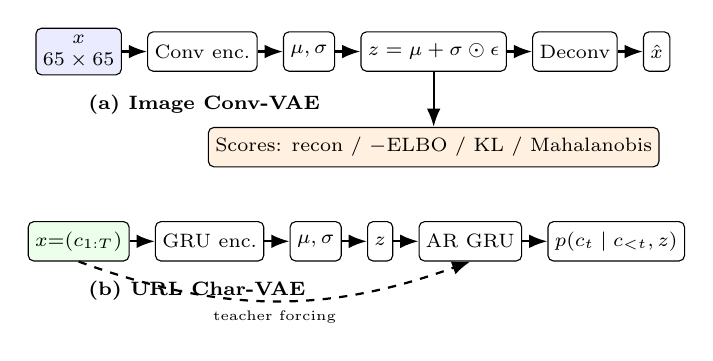
\begin{tikzpicture}[
    font=\scriptsize,
    box/.style={draw, rounded corners=2pt, align=center, inner sep=2.5pt, minimum height=0.5cm},
    arr/.style={-{Latex}, thick},
    node distance=0.28cm and 0.32cm
  ]
    \node[box, fill=blue!8] (xin) {$x$\\$65\times65$};
    \node[box, right=of xin] (enc) {Conv enc.};
    \node[box, right=of enc] (ms) {$\mu,\sigma$};
    \node[box, right=of ms] (z) {$z=\mu+\sigma\odot\epsilon$};
    \node[box, right=of z] (dec) {Deconv};
    \node[box, right=of dec] (xhat) {$\hat{x}$};
    \draw[arr] (xin) -- (enc);
    \draw[arr] (enc) -- (ms);
    \draw[arr] (ms) -- (z);
    \draw[arr] (z) -- (dec);
    \draw[arr] (dec) -- (xhat);
    \node[below=0.12cm of xin, font=\scriptsize\bfseries, anchor=north west] {(a) Image Conv-VAE};
    \node[box, fill=orange!12, below=0.7cm of z] (scores)
      {Scores: recon / $-\mathrm{ELBO}$ / KL / Mahalanobis};
    \draw[arr] (z.south) -- (scores.north);

    \node[box, fill=green!8, below=1.85cm of xin] (uin) {$x{=}(c_{1:T})$};
    \node[box, right=of uin] (uenc) {GRU enc.};
    \node[box, right=of uenc] (ums) {$\mu,\sigma$};
    \node[box, right=of ums] (uz) {$z$};
    \node[box, right=of uz] (udec) {AR GRU};
    \node[box, right=of udec] (uhat) {$p(c_t\mid c_{<t},z)$};
    \draw[arr] (uin) -- (uenc);
    \draw[arr] (uenc) -- (ums);
    \draw[arr] (ums) -- (uz);
    \draw[arr] (uz) -- (udec);
    \draw[arr] (udec) -- (uhat);
    \draw[arr, dashed] (uin.south) to[bend right=20]
      node[below, font=\tiny, pos=0.5] {teacher forcing} (udec.south);
    \node[below=0.12cm of uin, font=\scriptsize\bfseries, anchor=north west] {(b) URL Char-VAE};
  \end{tikzpicture}%
  }
  \caption{Model overview.
  (a)~Convolutional VAE on QR module grids with four anomaly scores.
  (b)~Character-level GRU VAE with autoregressive decoder and teacher forcing; $\beta$-annealed ELBO.}
  \label{fig:models}
\end{figure}

\subsection{Stage 2: Anomaly scores}
Orient every score so that larger values indicate greater anomaly.
For the image VAE, evaluate reconstruction loss, negative ELBO, KL divergence, and latent Mahalanobis distance.
Fit the latent mean $m$ and covariance $\Sigma$ using only benign training posterior means:
\begin{equation}
s_{\mathrm{latent}}(x)=(\mu_\phi(x)-m)^\top\Sigma^{-1}(\mu_\phi(x)-m).
\end{equation}
\pending{Specify covariance regularization and the latent-score convention.}

Deterministic reconstruction scores use $z=\mu_\phi(x)$ to avoid latent sampling noise.
For URLs, normalize by the number of nonpadding characters:
\begin{equation}
s_{\mathrm{URL-rec}}(x)=\frac{\ell_{\mathrm{URL}}(x,\mu_\phi(x))}{T}.
\end{equation}
A Monte Carlo negative-ELBO score at $\beta=1$ is
\begin{equation}
s_{\mathrm{NELBO}}(x)
=
\frac{1}{M}\sum_{k=1}^{M}\ell(x,z^{(k)})
+
\KL(q_\phi\|p),
\end{equation}
where $z^{(k)}\sim q_\phi(z\mid x)$.
For URL reporting, divide this entire score by $T$.
A reconstruction-plus-KL score evaluated solely at the posterior mean is a deterministic surrogate, not the exact expected negative ELBO.
\pending{Fix $M$, evaluation random seeds, and whether the final report uses a Monte Carlo score, a deterministic surrogate, or both.}

\subsection{Stage 3: Feature floors and supervised references}
Fit each feature floor on benign training examples.
With a single feature $f$, use the absolute standardized deviation
\begin{equation}
s_{\mathrm{floor}}(x)=\left|\frac{f(x)-m_f}{\sigma_f}\right|.
\end{equation}
For multiple features, use Mahalanobis distance from their benign mean.
The absolute deviation is needed because both unusually short and unusually long URLs can differ from benign examples.
Table~\ref{tab:floors} specifies the planned comparisons.

\begin{table}[t]
\centering
\caption{Benign-only feature floors and supervised references.}
\label{tab:floors}
\small
\begin{tabularx}{\linewidth}{p{1.05in}Y}
\toprule
Comparison & Inputs and training information \\
\midrule
Image floors A/B & Modules per side and dark-pixel fraction; A and B are identical in the current plan. \\
URL floor A & URL length only. \\
URL floor B & URL length, has-scheme flag, IP-host flag, host-label count, path length, and digit ratio. \\
Image reference & Matching convolutional encoder architecture plus one linear binary-classification head. \\
URL reference & Matching GRU encoder architecture plus one linear binary-classification head. \\
\bottomrule
\end{tabularx}
\end{table}

Supervised references train from scratch on labeled benign and malicious training items.
They reuse the encoder architecture and are fitted independently.
A sigmoid converts the classifier logit to a malicious-class probability.
These references show what labels and malicious examples add; they are not an upper bound because their training information and sample counts differ from those of the VAEs.

%==============================================================================
\section{Training Procedure}
%==============================================================================

\subsection{Training data and configuration selection}
Train VAEs and feature floors only on benign training items.
Train supervised references on both labeled classes within the same training partition.
Malicious examples are restricted to evaluation for the VAEs; use benign validation objectives and collapse diagnostics for their configuration selection.
Select latent size, KL weight, likelihood, and optimization settings before evaluating the test set.
Do not use malicious test items for model or score selection.
\pending{Clarify whether labeled malicious validation items are used to select the headline score or any VAE configuration. If they are used, disclose that validation-label use explicitly and revise the stated benign-only selection protocol.}

\subsection{Optimization and KL annealing}
Log reconstruction loss, KL, and the full weighted objective against iterations or epochs.
For the URL model, anneal $\beta$ from near zero to the target value and inspect whether the latent variable remains informative.
Loss reduction and Gaussian variance scaling must be documented because they change the balance between reconstruction and KL.
Table~\ref{tab:config} retains unresolved implementation settings.

\begin{table}[t]
\centering
\caption{Training configuration to finalize before test evaluation.}
\label{tab:config}
\small
\begin{tabularx}{\linewidth}{p{1.15in}YY}
\toprule
Setting & Image VAE & URL VAE \\
\midrule
Input & $65\times65$ grid & Up to 256 characters \\
Likelihood & Bernoulli or Gaussian & Categorical \\
Latent dimension & Pending & Pending \\
Encoder/decoder width & Pending & Pending \\
Optimizer and learning rate & Pending & Pending \\
Batch size and epochs & Pending & Pending \\
Target $\beta$ and schedule & Pending & Pending \\
Checkpoint rule & Pending & Pending \\
Training seeds & At least 5 & At least 5 \\
\bottomrule
\end{tabularx}
\end{table}

\subsection{Repeated runs and reproducibility}
Vary latent size, $\beta$, and likelihood one at a time on validation data, then run the selected configuration with at least five training seeds.
Keep splits and feature extraction fixed across seeds and models.
Save the chosen checkpoint, configuration, training history, and per-item scores.
\pending{Add hardware, software versions, exact seeds, training time, checkpoint criterion, and the completed validation-search record.}

%==============================================================================
\section{Evaluation Metrics}
%==============================================================================

\subsection{Ranking quality and class prevalence}
Report AUROC and AUPRC with malicious items as the positive class.
AUROC summarizes ranking and equals 0.5 for a random scorer.
AUPRC depends on prevalence: with approximately 57\% malicious items, its no-skill reference is approximately 0.57.
Report the actual evaluation-cohort prevalence next to each AUPRC.
\pending{State whether the implementation computes average precision or an interpolated PR-curve area.}

\subsection{Recall at low false-positive rates}
For target FPR $\alpha\in\{0.01,0.05\}$, obtain a threshold only from benign validation scores, using the empirical $(1-\alpha)$ quantile.
Flag items with scores above the threshold, and report both recall and the achieved test FPR.
The calibration target does not guarantee that test FPR equals $\alpha$ under domain shift.
\pending{Specify quantile interpolation, tie handling, and score-specific thresholds.}

\subsection{Domain bootstrap and seed variability}
Compute 95\% bootstrap confidence intervals by resampling whole domains, preserving within-domain correlations.
For the VAE-minus-floor AUROC difference, apply the same resampled domains to both models so the comparison remains paired.
Report mean and spread across at least five training seeds and keep seed variability distinct from bootstrap uncertainty for a fixed model.
\pending{Fix bootstrap repetitions, interval method, class-degenerate replicate handling, and the rule for combining or reporting seed and sampling uncertainty.}

\subsection{Stratified evaluation}
Report AUROC by QR version, treating Micro QR as a separate image stratum, and by URL-length bin and URL scheme for the URL model.
Include counts for both classes in every stratum.
Freeze bin edges and the criterion for sufficient sample size on validation data.
The IP-host group is reported by class share rather than AUROC because benign IP hosts are extremely sparse in the supplied EDA.

\subsection{Success criteria}
Apply the following criteria separately to each VAE:
\begin{itemize}
  \item \textbf{Beyond the headline floor:} the paired 95\% CI for test AUROC minus that modality's floor-A AUROC lies above zero. Report floor~B alongside it.
  \item \textbf{Within strata:} the same difference is positive with a CI above zero in a majority of prespecified eligible strata; report every stratum and any exclusions.
  \item \textbf{Across seeds:} the lowest-AUROC seed still exceeds the headline floor under the prespecified robustness rule~\citep{bouman}.
\end{itemize}
\pending{Fix the eligible-stratum minimum and whether the lowest-seed criterion requires a positive point difference or a CI above zero.}

As a descriptive measure, report the fraction of the floor-to-supervised-reference AUROC gap closed by the VAE:
\begin{equation}
g=\frac{A_{\mathrm{VAE}}-A_{\mathrm{floor}}}{A_{\mathrm{reference}}-A_{\mathrm{floor}}}.
\end{equation}
Here $A$ denotes AUROC on the same items.
Report $g$ as undefined if the denominator is zero, and interpret it cautiously if the reference does not exceed the floor.
It is descriptive, without a success threshold.

%==============================================================================
\section{Experimental Results}
%==============================================================================

\subsection{Completed preliminary EDA}
Table~\ref{tab:eda} records EDA quantities from the proposal and notes.
These are descriptive findings, not VAE detection results.
Figures~\ref{fig:size} and~\ref{fig:url} show the corresponding EDA plots.

\begin{table}[t]
\centering
\caption{Preliminary EDA from the project materials. Percentages are approximate.}
\label{tab:eda}
\small
\begin{tabular}{lrr}
\toprule
Quantity & Benign & Malicious \\
\midrule
URLs with no scheme & 91\% & 37\% \\
IP-address host & 0.006\% & 26\% \\
URLs exceeding 256 characters & 0.04\% & 1.0\% \\
Fits $65\times65$ canvas (sample) & 99.9\% & 99.3\% \\
\bottomrule
\end{tabular}
\end{table}

The proposal's plots show that QR module size closely follows URL length.
Notes additionally describe malicious URL lengths as having a shorter median but a longer tail than benign lengths; exact medians and quantiles were not supplied.
Together with the scheme and IP-host differences, this motivates two-sided feature-distance floors and within-stratum comparisons.

\begin{figure}[t]
\centering
\figureorbox{eda_qr_size.png}{\textbf{Missing \texttt{eda\_qr\_size.png}.} QR module-size distributions, size over-representation by class, and QR size vs.\ URL length.}
\caption{QR size and URL-length relationship: module-size distributions by class, class over-representation by module size, and QR size against URL length.
This figure reports data properties rather than model performance.}
\label{fig:size}
\end{figure}

\begin{figure}[t]
\centering
\figureorbox{eda_url_structure.png}{\textbf{Missing \texttt{eda\_url\_structure.png}.} URL schemes and structural flags by class.}
\caption{URL schemes and structural flags by class.
Malicious URLs more often carry an explicit scheme and an IP-address host; the logarithmic structural-flag axis makes rare benign properties visible.}
\label{fig:url}
\end{figure}

\subsection{Main model comparison}
No completed VAE, floor, or supervised-reference metrics are available yet.
Table~\ref{tab:results} provides the final reporting structure without fabricating results.
All rows within a modality must use the same eligible test items.
\pending{Fill with completed metrics, domain-bootstrap intervals, seed summaries, test counts, prevalence, and achieved FPRs.}

\begin{table}[t]
\centering
\caption{Planned test comparison.
Dashes denote missing results.
R@1/R@5 are recall at thresholds calibrated to 1\%/5\% benign validation FPR; $\Delta$A is AUROC minus floor A.}
\label{tab:results}
\small
\begin{tabular}{llccccc}
\toprule
Modality & Model/score & AUROC & AUPRC & R@1 & R@5 & $\Delta$A \\
\midrule
QR & Feature floor A (= B) & \missing & \missing & \missing & \missing & -- \\
QR & VAE reconstruction & \missing & \missing & \missing & \missing & \missing \\
QR & VAE negative ELBO & \missing & \missing & \missing & \missing & \missing \\
QR & VAE KL & \missing & \missing & \missing & \missing & \missing \\
QR & VAE latent distance & \missing & \missing & \missing & \missing & \missing \\
QR & Supervised CNN reference & \missing & \missing & \missing & \missing & \missing \\
\midrule
URL & Feature floor A (length) & \missing & \missing & \missing & \missing & -- \\
URL & Feature floor B (six features) & \missing & \missing & \missing & \missing & \missing \\
URL & VAE NLL/character & \missing & \missing & \missing & \missing & \missing \\
URL & VAE negative ELBO/character & \missing & \missing & \missing & \missing & \missing \\
URL & Supervised GRU reference & \missing & \missing & \missing & \missing & \missing \\
\bottomrule
\end{tabular}
\end{table}

\subsection{Learning objective versus iterations}
\begin{figure}[t]
\centering
\figureorbox{elbo_curves.png}{\pending{Figure: ELBO training curves.}\\
Image and URL VAEs: negative ELBO, reconstruction, and KL vs.\ training iterations (train and validation); overlay the $\beta$ schedule for the URL model.
Save as \texttt{elbo\_curves.png}.}
\caption{Learning objective as a function of training iterations for both VAEs.}
\label{fig:elbo}
\end{figure}
\pending{Describe convergence, the train/validation gap, and whether the URL KL term stays above zero after annealing.}

\subsection{Visualization of the learned model}
\begin{figure}[t]
\centering
\figureorbox{recon_latent.png}{\pending{Figure: reconstructions, samples, latent structure.}\\
(a)~Test QR images, reconstructions, and pixel-error maps (benign vs.\ malicious).
(b)~Samples decoded from $z\sim\mathcal{N}(0,I)$.
(c)~2D t-SNE or PCA of latent means $\mu(x)$, colored by class and QR version.
Save as \texttt{recon\_latent.png}.}
\caption{Learned image-VAE structure: reconstructions, prior samples, and latent embeddings.}
\label{fig:viz}
\end{figure}

\subsection{Ablations and training diagnostics}
\pending{Report validation comparisons for latent dimension, target KL weight, and image likelihood. Identify any collapsed URL runs. State the configuration chosen before test evaluation.}

\subsection{Stratified and multi-seed results}
\pending{Add per-stratum class counts, VAE/floor AUROC and paired confidence intervals, at least five per-seed results, and the descriptive supervised-gap measure. State whether each prespecified success criterion is met.}

\subsection{Qualitative reconstructions and error cases}
\pending{Show representative benign and malicious QR reconstructions, high- and low-scoring URL examples, and missed anomalies that reconstruct well. Describe the sample-selection rule and relate examples to size, scheme, and domain strata.}

%==============================================================================
\section{Analysis and Discussion}
%==============================================================================

\paragraph{Why simple feature floors matter.}
EDA shows large differences in URL scheme and host type, while QR size tracks URL length.
An aggregate score can separate the two classes using these properties alone.
The feature floors establish how much of this signal is available without a learned image or sequence representation.
\pending{Compare each completed VAE score to both floors and explain the paired AUROC differences.}

\paragraph{Reconstruction is not a benignness guarantee.}
A model trained on benign data can reconstruct a malicious input accurately~\citep{bouman}.
KL regularization and latent-distance scoring offer additional views but do not eliminate this failure mode.
\pending{Use actual false negatives and score comparisons to assess whether malicious items reconstruct well, occupy typical benign latent regions, or differ only through the KL contribution.}

\paragraph{What the two modalities capture.}
The URL model observes lexical sequences; the image model observes how a payload is encoded into modules.
Comparisons on paired items can reveal whether either representation adds discrimination after length and QR-version controls.
The deterministic relationship between payload and render limits claims that they are independent evidence sources.
\pending{Discuss agreement and disagreement between image and URL scores on the same test cohort.}

\paragraph{Domain grouping and generalization.}
Random splitting can place related URLs from the same domain in training and test.
Grouping makes the intended question more demanding: can the score generalize to unseen domains?
The large reported random-split overlap motivates this control, but the inconsistent grouped-overlap figures must be resolved.
\pending{Report the final leakage audit and interpret performance on held-out domains without claiming guarantees for all future threats.}

\paragraph{Posterior collapse and seed robustness.}
Near-zero KL can indicate that the decoder ignores the latent variable, especially when URL character context is predictive.
A favorable mean score can also conceal weak seeds.
\pending{Interpret the KL traces, annealing comparisons, per-seed spread, and worst-seed result together. Avoid inferring useful latent information from reconstruction quality alone.}

\paragraph{Interpreting the success criteria.}
Exceeding the declared floor within eligible strata supports a narrower conclusion: the model uses information beyond the tested features.
It does not identify malicious intent, rule out unmeasured shortcuts, or show that every anomaly will be detected.
Failing the criteria is also a meaningful result about benign-only generative detection in this dataset.
\pending{State the conclusion justified by the final comparisons, including negative or mixed findings.}

%==============================================================================
\section{Limitations and Future Work}
%==============================================================================

\paragraph{Synthetic images and dataset construction.}
Synthetic renders omit blur, rotation, lighting, damage, overlays, and camera perspective.
Performance on these images cannot establish robustness to physical QR codes.
Dataset collection and rendering choices may introduce class differences beyond maliciousness.
Future work should test separate data sources and photographed codes with an explicit external evaluation protocol.

\paragraph{Coverage and input restrictions.}
The $65\times65$ canvas excludes large grids, and 256-character truncation removes more malicious than benign URL tails according to EDA.
These choices change which items can be modeled and what information remains.
Report full exclusion counts and test sensitivity to larger inputs before generalizing beyond the eligible cohort.

\paragraph{Generative blind spots and operating thresholds.}
VAEs need not assign lower likelihood to every malicious example.
Benign validation thresholds may also yield different FPRs on new domains or under changing prevalence and collection conditions.
Multiple scores and bootstrap intervals characterize observed behavior rather than resolving those blind spots.

\paragraph{Remaining experiments.}
\pending{Complete and document the split audit, model training, feature floors, supervised references, score definitions, held-out evaluation, seed study, ablations, and qualitative analysis. Add measured compute cost and any limitations revealed by the completed experiments.}

%==============================================================================
\section*{Team Contributions}
%==============================================================================

\noindent\textbf{Joe Nguyen.} \pending{Add verified contribution.}\\
\noindent\textbf{Adithya Rajendra.} \pending{Add verified contribution.}\\
\noindent\textbf{Anishwar Chakraborty.} \pending{Add verified contribution.}\\
\noindent\textbf{Atharva Deshpande.} \pending{Add verified contribution.}\\
\noindent\textbf{Swaroop Veerla.} \pending{Add verified contribution.}\\
\pending{Confirm shared literature-review, writing, audit, and integration contributions.}

\section*{Code and Reproducibility}
\pending{Add repository URL, commit, tested commands, and artifact locations.}
Release the dataset version/filtering ledger, paired domain-grouped splits, preprocessing and model/floor settings, training configurations, seeds, checkpoints, per-item scores, calibrated thresholds, bootstrap settings, and hardware/software requirements.

\bibliographystyle{plainnat}
\bibliography{references}

\end{document}
